\documentclass[jou]{apa6}

\usepackage[american]{babel}

\usepackage{csquotes}
\usepackage[style=apa,sortcites=true,sorting=nyt,backend=biber]{biblatex}
\DeclareLanguageMapping{american}{american-apa}
\addbibresource{bibliography.bib}


%%%%%%%%%%%%%%%%%%%%%%%%%%%%%%%%%%%%%%%%
%% Discrete Structures
%% The start of RBS stuff
%%%%%%%%%%%%%%%%%%%%%%%%%%%%%%%%%%%%%%%%

% Working internal and external links in PDF
\usepackage{hyperref}
% Extra math symbols in LaTeX
\usepackage{amsmath}
\usepackage{gensymb}
\usepackage{amssymb}
% Enumerations with (a), (b), etc.
\usepackage{enumerate}
\usepackage[framemethod=TikZ]{mdframed}
\usepackage{xcolor}
\usepackage{graphicx}
\usepackage[justification=centering]{caption}
\usepackage{fancyvrb}
\usepackage{standalone}
\usepackage{xcolor}

\let\OLDitemize\itemize
\renewcommand\itemize{\OLDitemize\addtolength{\itemsep}{-6pt}}

\usepackage{etoolbox}
\makeatletter
\preto{\@verbatim}{\topsep=3pt \partopsep=3pt }
\makeatother

% These sizes redefine APA for A4 paper size
\oddsidemargin 0.0in
\evensidemargin 0.0in
\textwidth 6.27in
\headheight 1.0in
%\topmargin -24pt
\topmargin -32pt
\headheight 12pt
\headsep 12pt
%\textheight 9.19in
\textheight 9.35in


\title{Sample Quiz 8}
\author{Discrete Structures, Spring 2020}
\affiliation{RBS}

\leftheader{Discrete Sample Quiz 8}

\abstract{%
}

%\keywords{}

\setlength\parindent{0pt}
\begin{document}


\thispagestyle{empty}

\twocolumn
\begin{center}
{\large \bf Discrete Structures, Homework 3}
\end{center}


Submit a PDF file to ORTUS by 2020-03-16.

\vspace{4pt}
{\bf Problem 1 (Rosen2019, \#33, p.444)} \textendash{} {\em After 6.4.}\\
Prove that if $n$ is a positive integer, then 
${\displaystyle \sum\limits_{k=1}^n k \cdot{} {n \choose k} = n \cdot{} 2^{n-1}}$. 

\vspace{8pt}
{\bf Problem 2 (Rosen2019, \#48, p.456)} \textendash{} {\em After 6.5.}\\
A shelf holds $12$ books in a row. How many ways are there to choose five books so that no two adjacent books 
are chosen?

\vspace{8pt}
{\bf Problem 3 (Rosen2019, \#16, p.464)} \textendash{} {\em After Ch.6.}\\
Show that in any set of $n+1$ positive integers not exceeding $2n$ there must be two 
that are relatively prime.

\vspace{8pt}
{\bf Problem 4 (Rosen2019, \#33, p.465)} \textendash{} {\em After Ch.6.}\\
How many bit strings of length $n$, where $n \geq 4$, contain exactly two 
occurrences of {\tt 01}.

\vspace{8pt}
{\bf Problem 5 (Miller2014, Exercise1.18 \url{https://bit.ly/2TfZErQ})} {\em The Theory and Applications of 
Benford's Law. Steven J. Miller (editor).}\\
Compute the values of this function $f(x) = \left| x^2 \cdot \tan x \right|$ for 
all integers $x \in \{ 1,\ldots,100000 \}$. Record the very first digit that appears in every value $f(x)$.\\
{\bf (A)} What is the ratio of the digit {\tt 1} among these $10^5$ digits (empirical probability)?\\
{\bf (B)} What is the theoretical ratio of the first digit {\tt 1} predicted by the Benford's law? 

{\em Note.} Benford's Law is routinely checked by people who falsify the results of elections 
or otherwise fabricate large amounts of data. 
Generating digits with the uniform random distribution (where each 
digit has the same chance to appear) would create data sets that look highly artificial
when statistically examined.

\vspace{8pt}
{\bf Problem 6 (Rosen2019, \#23, p.503)} \textendash{} {\em After 7.3.}\\
Suppose that $E_1$ and $E_2$ are the events that an incoming mail message contains the words
$w_1$ and $w_2$, respectively. 
Assuming that $E_1$ and $E_2$ are independent events and that $(E_1 \,\mid\, S)$ 
and $(E_2 \,\mid\, S)$ are independent events, 
where $S$ is the event that an incoming message is spam, and that we have 
no prior knowledge regarding whether or not the message is spam, show that


$$P\left( S \,\mid\, E_1 \cap E_2 \right) =$$
$$= \frac{P(E_1 \,\mid\, S) \cdot P(E_2 \,\mid\, S)}{P(E_1 \,\mid\, S) \cdot P(E_2 \,\mid\, S)
+ P(E_1 \,\mid\, \overline{S} ) \cdot P(E_2 \,\mid\, \overline{S} )}.$$

\vspace{8pt}
{\bf Problem 7 (Rosen2019, \#39, p.519)} \textendash{} {\em After 7.4.}\\
Suppose that the number of aluminum cans recycled in a day at a recycling center
is a random variable with an expected value of $50000$ and a variance of $10000$.\\
{\bf (A)} Use Markov's inequality (Exercise 37) to find an upper bound 
on the probability that the center will recycle more than $55000$ cans on a particular day.\\
{\bf (B)} Use Chebyshev's inequality to provide a lower bound on the probability that the center
will recycle $40000$ to $60000$ cans on a certain day.

\vspace{8pt}
{\bf Problem 8 (Rosen2019, \#15, p.522)} \textendash{} {\em After Ch.7.}\\
Suppose that $m$ and $n$ are positive integers. What is the probability that 
a randomly chosen positive integer less than $mn$ 
is not divisible by either $m$ or $n$? 

\vspace{8pt}
{\bf Problem 9 (Rosen2019, \#22, p.523)} \textendash{} {\em After Ch.7.}\\
Suppose that $n$ balls are tossed into $b$ bins so that each 
ball is equally likely to fall into any of the bins and that the tosses are independent.\\
{\bf (A)} Find the probability that a particular ball lands in a specified bin.\\
{\bf (B)} What is the expected number of balls that land in a particular bin.\\
{\bf (C)} What is the expected number of balls tossed until a particular bin contains a ball?\\
{\bf (D)} What is the expected number of balls tossed until all bins contain a ball?\\
{\em Hint:} Let $X_i$ denote the number of tosses required to have a ball land in 
the $i$th bin once $i-1$ bins contain a ball. Find $E(X_i)$ and use the linearity of 
expectations.

\vspace{8pt}
{\bf Problem 10 (Rosen2019, \#30, p.524)} \textendash{} {\em After Ch.7.}\\
Use Chebyshev's inequality to show that the probability that more than $10$ people get the 
correct hat back when a hatcheck person returns hats at random does not exceed $1/100$
no matter how many people check their hats.\\
{\em Hint.} See Example 6, (Rosen2019, p.507) about the random hat assigning experiment 
and Exercise 43, (Rosen2019, p.520) about the fixed elements in a random permutation.







\newpage

\section{Answers}

\vspace{4pt}
{\bf Problem 1}\\
We can apply the first derivative to the expression $y = (1+x)^n$: 
$$y' = n \cdot (1 + x)^{n-1}.$$
If we plug in the value $x = 1$, we would get 
\begin{equation}
\label{eq:expr11}
y'(1) = n \cdot 2^{n-1}.
\end{equation}
On another hand, we can also expand the expression for $(1+x)^n$ using
the binomial formula and only then compute its derivative. 
$$y = {n \choose 0} 1 + {n \choose 1} x^1 + {n \choose 2} x^2 + \ldots + {n \choose n} x^n.$$
Now compute it as a derivative of a sum: 
$$y' = 0 + {n \choose 1} x^0 + 2 \cdot {n \choose 2} x^1 + \ldots + n \cdot {n \choose n} x^{n-1}.$$
Substituting $x=1$ again we get that 
\begin{equation}
\label{eq:expr12}
y'(1) = \sum\limits_{k=1}^n k \cdot {n \choose k}.
\end{equation}
We expressed $y'(1)$ in two different ways in (\ref{eq:expr11}) and (\ref{eq:expr12}), so they must be equal:
$$\sum\limits_{k=1}^n k \cdot{} {n \choose k} = n \cdot{} 2^{n-1}.$$

\vspace{10pt}
{\bf Problem 2}\\
Denote by $n_0$, $n_1+1$, $n_2+1$, $n_3+1$, $n_4+1$, $n_5$ the numbers of those books that are {\bf not}
chosen. In particular, $n_0$ is the number of books to the left of all chosen books; 
$n_1+1$ is the number of books between the first and the second chosen book, etc. 
Finally, $n_5$ is the number of books to the right of all five books. 
Since no two books are adjacent, all the $n_1+1,\ldots,n_4+1$ are strictly positive. 
Therefore, $n_0,n_1,n_2,n_4,n_5$ are all nonnegative. 

We also know that $n_0 + n_1 + n_2 + n_4 + n_5 = 3$. The number of non-negative solutions
for this integer equation with six variables is known as 
the {\em combination with repetitions}, where we select exactly $k=3$ items out of a
set of $n=6$ different elements (for example, we make an unordered ``handful'' of three balls, 
where each ball can be in  any of six colors). 

The formula to compute combination with repetitions is this:
$${n+k-1 \choose k} = {6+3-1 \choose 3} = {8 \choose 3} = \frac{8!}{3!\,5!} = 56.$$

\vspace{10pt}
{\bf Problem 3}\\
Split all $2n$ integers into pairs $(1;2)$, $(3;4)$, $\ldots$, $(2n-1;2n)$. 
Since we  choose $n+1$ positive integers and there are  only $n$ pairs, 
by Pigeonhole principle there will be two selected numbers from the same
pair. Denote them by $(2k-1;2k)$. 

It is easy to see that two adjacent numbers $2k-1$ and $2k$ must be 
mutually prime, since any common divisor $d$ for both of them 
is also a divisor of their difference $2k - (2k-1) = 1$. 
Therefore $d = \pm 1$. 


\vspace{10pt}
{\bf Problem 4}\\
Let us represent the sequence of $n$ bits (containing exactly two 
substrings $\textcolor{red}{\mathtt{01}}$) split into eight consecutive chunks \textendash{}
all but two of them can be empty: 
$$\underbrace{1\ldots{}1}_{n_1}\underbrace{0\ldots{}0}_{n_2}\textcolor{red}{\mathtt{01}}
\underbrace{1\ldots{}1}_{n_3}\underbrace{0\ldots{}0}_{n_4}\textcolor{red}{\mathtt{01}}
\underbrace{1\ldots{}1}_{n_5}\underbrace{0\ldots{}0}_{n_6}.$$

There are two chunks to the left of the first instance of $\textcolor{red}{\mathtt{01}}$; 
at first there are any number $n_1\geq 1$ of ``ones'', followed by any number of 
$n_2 \geq 0$ ``zeroes''. Then come exactly two digits $\textcolor{red}{\mathtt{01}}$; and then 
the pattern repeats itself \textendash{} some $n_3$ ``ones'', $n_4$ ``zeroes'', 
then there are another two digits $\textcolor{red}{\mathtt{01}}$, then again 
$n_5$ ``ones'' and $n_6$ ``zeroes''.

We claim that {\bf any} string satisfying the condition of the problem looks 
in this way (perhaps, some of $n_i$ can be equal to $0$ and thus the corresponding digits will be absent).
Any situation, where some digits ``zeroe'' are followed by ``one'' would result to 
more instances of $\textcolor{red}{\mathtt{01}}$. 

We must therefore find the number of non-negative solutions for the following integer 
equation: 
$$n_1 + n_2 + n_3 + n_4 + n_5 + n_6 = n-4.$$
Their sum equals $n-4$ because two pairs of $\textcolor{red}{\mathtt{01}}$ are removed from a 
sequence of exactly $n$ bits. 
The number of solutions equals the {\em combinations with repetition} where we 
select a ``handful'' of $n-4$ items, where every item can be in any of $6$ colors. 

We can represent this as a problem to arrange $n-4$ circles with $5$ separators. 
The total number os such arrangements is expressed with the formula of combinations with repetition: 
$${(n-4) + 5 \choose 5} = {n+1 \choose 5} = \frac{(n+1)n(n-1)(n-2)(n-3)}{5!}.$$
We can show the number of such sequences $S_n$ for some small $n$ in this table:

\begin{tabular}{|l|r|r|r|r|r|r|r|r|} \\ \hline
$n$   & $4$ & $5$ & $6$  & $7$  & $8$   & $9$   & $10$ & $11$ \\ \hline
$S_n$ & $1$ & $6$ & $21$ & $56$ & $126$ & $252$ & $462$ & $792$ \\ \hline
\end{tabular}


\vspace{10pt}
{\bf Problem 5}\\

{\bf (A)} We can compute all the values of the function $|x^2 \cdot \tan x|$
and extract all the first digits. 
We get exactly $29904$ members of the digit sequence (out of 
$100000$) that are equal to $1$. 

{\bf (B)} Benford's distribution is computed using
the formula 
$$P(d) = \log_{10} (d+1) - \log_{10} d,$$
where $d=1,\ldots,9$. In particular, 
$P(\mathtt{1}) = 0.30103$. 
The empirical distribution of all the first digits 
and also the theoretical (Benford) distribution is shown in the table. 


\begin{tabular}{|l|l|l|} \hline
Digit & Empirical & Benford \\ \hline
$1$ & $29904$ & $0.30103$ \\ \hline
$2$ & $17514$ & $0.17609$ \\ \hline
$3$ & $12479$ & $0.12494$ \\ \hline
$4$ & $9718$ & $0.09691$ \\ \hline
$5$ & $8006$ & $0.07918$ \\ \hline
$6$ & $6776$ & $0.06695$ \\ \hline
$7$ & $5871$ & $0.05799$ \\ \hline
$8$ & $5146$ & $0.05115$ \\ \hline
$9$ & $4586$ & $0.04576$ \\ \hline
\end{tabular}

\begin{figure}[!htb]
\center{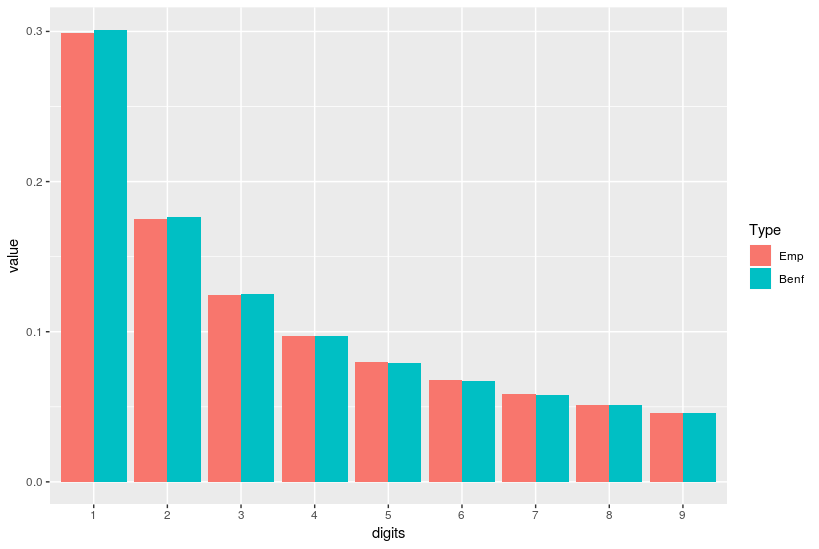
\includegraphics[width=3in]{hw03/benford.png}}
\caption{\label{fig:benford} Empirical and Benford distributions.}
\end{figure}

{\em Note.} As we see the empirical distribution is very close
to the Benford's distribution. This has nothing to do with 
any particular properties of the function $|x^2 \cdot \tan x|$
(besides the fact that this function takes all kinds of large values). 



\vspace{10pt}
{\bf Problem 6}\\
Note that the formula (\ref{eq:wrong-bayes}) that you have to prove is wrong:

\begin{align}
 & P\left( S \,\mid\, E_1 \cap E_2 \right) = \nonumber \\
= & \frac{P(E_1 \,\mid\, S) \cdot P(E_2 \,\mid\, S)}{P(E_1 \,\mid\, S) \cdot P(E_2 \,\mid\, S)
+ P(E_1 \,\mid\, \overline{S} ) \cdot P(E_2 \,\mid\, \overline{S} )}. \label{eq:wrong-bayes}
\end{align}


To see that it is wrong, assume that the conditional probabilities $P(E_i \,\mid\, S)$
and $P(E_i \,\mid\, \overline{S})$ do not differ very much, but the probability of spam is very low: 
$P(S) << P(\overline{S})$. In this case we should get that $P\left( S \,\mid\, E_1 \cap E_2 \right)$ 
is also very small (because the events $E_1$, $E_2$ do not provide any useful evidence), but
spam is very unlikely. On the other hand, the formula would imply that the probability of spam is around $1/2$, 
since we assumed that $P(E_1 \,\mid\, S) \approx P(E_1 \,\mid\, \overline{S})$
and $P(E_2 \,\mid\, S) \approx P(E_2 \,\mid\, \overline{S})$, so the denominator is about two times larger
than the numerator. In the textbook this was caused by an assumption that 
$P(S) = P(\overline{S}) = \frac{1}{2}$; see (Rosen2019, p.498). 


Let us obtain and prove a correct formula. 
Apply the (regular) Bayes formula for the conditional probability of spam event $S$, assuming that 
the event $E_1 \cap E_2$ already holds. We get this:
\begin{align}
 & P\left( S \,\mid\, E_1 \cap E_2 \right) = \nonumber \\
= & \frac{P((E_1 \cap E_2) \,\mid\, S) \cdot P(S)}{P((E_1 \cap E_2) \,\mid\, S) \cdot P(S)
+ P((E_1 \cap E_2) \,\mid\, \overline{S}) \cdot P(\overline{S})}. \label{eq:bayes1}
\end{align}



The notation $(E_1 \mid S) \cap (E_2 \mid S)$ means that in the event universe $S$ 
(``assuming the spam event $S$ already holds'')
both the event $E_1$ and $E_2$ have happened. Therefore
\begin{align}
 & P((E_1 \cap E_2) \mid S) = \nonumber \\
= & P((E_1 \mid S) \cap (E_1 \mid S)) = P(E_1 \mid S) \cdot P(E_2 \mid S) \label{eq:indep1}
\end{align}
The first equality rewrites the intersection $E_1 \cap E_2$ in the 
conditional event space (assuming that $S$ has already happened).
The second equality holds, because 
it was known that $(E_1 \mid S)$ and $(E_2 \mid S)$ are mutually independent. 

Similar identities hold in the complementary conditional event space 
(assuming that $\overline{S}$ has happened and this is not a spam): 
\begin{align}
 & P((E_1 \cap E_2) \mid \overline{S}) = \nonumber \\
= & P((E_1 \mid \overline{S}) \cap (E_1 \mid \overline{S})) = 
P(E_1 \mid \overline{S}) \cdot P(E_2 \mid \overline{S}) \label{eq:indep2}
\end{align}
Indeed, if the last equality in (\ref{eq:indep2}) would not hold, then we would get 
\begin{align}
 & P(E_1 \cap E_2) = P((E_1 \cap E_2) \mid S) + P((E_1 \cap E_2) \mid \overline{S}) \neq \nonumber \\
\neq &  P(E_1 \mid S) \cdot P(E_2 \mid S) + P(E_1 \mid \overline{S}) \cdot P(E_2 \mid \overline{S}) = \nonumber \\
= & P(E_1) \cdot P(E_2) \label{eq:indep3}
\end{align}
This would contradict the fact that $E_1$ and $E_2$ are independent (in the original event space).

In other words, both events $(E_1 \mid \overline{S})$ and $(E_2 \mid \overline{S})$ should also be independent. Therefore: 
\begin{align}
 & P((E_1 \cap E_2) \mid \overline{S}) = \nonumber \\
= & P((E_1 \mid \overline{S}) \cap (E_1 \mid \overline{S})) = P(E_1 \mid \overline{S}) \cdot P(E_2 \mid \overline{S}) \nonumber 
\end{align}

Now we can rewrite the Bayes formula from (\ref{eq:bayes1}) and it completes the proof.

{\footnotesize
\begin{align}
 & P\left( S \,\mid\, E_1 \cap E_2 \right) = \nonumber \\
= & \frac{P((E_1 \cap E_2) \,\mid\, S) \cdot P(S)}{P((E_1 \cap E_2) \,\mid\, S) \cdot P(S)
+ P((E_1 \cap E_2) \,\mid\, \overline{S}) \cdot P(\overline{S})} = \nonumber \\
= & \frac{P(E_1 \,\mid\, S) \cdot P(E_2 \,\mid\, S) \cdot P(S)}{P(E_1 \,\mid\, S) \cdot P(E_2 \,\mid\, S) \cdot P(S)
+ P(E_1 \,\mid\, \overline{S} ) \cdot P(E_2 \,\mid\, \overline{S} ) \cdot P(\overline{S})}. \label{eq:bayes-correct}
\end{align}
}

Formula (\ref{eq:bayes-correct}) is always correct. It becomes (\ref{eq:wrong-bayes}) only 
if $P(S) = P(\overline{S}) = \frac{1}{2}$; in this case these factors can be cancelled.
(In the context of the given problem this would mean that there are equal number of 
known spam messages and also non-spam messages used to train the spam-detection
machine learning algorithm.)






\vspace{8pt}
{\bf Problem 7}\\
{\bf (A)} We know that $X \geq 0$ (there are no negative numbers of cans); 
and the mean value of processed cans is $E(X) = 50000$. 
By Markov's inequality we get for any $a>0$:
\begin{equation}
\label{eq:markov}
P(X \geq a) \leq \frac{E(X)}{a}.
\end{equation}
We can replace $a = 55000$, and get: 
$$P(X \geq 55000) \leq \frac{50000}{55000} = \frac{10}{11} = 0.9090909.$$

The problem actually asks, what is the probability that {\bf more} than 
$55000$ cans will be processed. We can estimate:
$$P(X > 55000) \leq P(X \geq 55000) \leq \frac{10}{11}.$$
Namely, the probability is {\bf at least} $\frac{10}{11}$. 
We cannot get any better estimate, since we could 
have $P(X = 55000) = 0$, and then $P(X > 55000) = P(X \geq 55000)$. 

{\em Note.} We could 
claim a slightly better inequality, since $P(X > 55000)$
for integer number of cans means that $P(X \geq 55001)$ and
by (\ref{eq:markov}) where $a = 55001$ we would 
$$P(X \geq 55001) \leq \frac{50000}{55001} = 0.9090744.$$

\vspace{4pt}
{\bf (B)} Chebyshev's inequality is this:
\begin{equation}
\label{eq:chebyshev}
P(|X-E(X)| \geq r) \leq \frac{V(X)}{r^2}.
\end{equation}
If we plug in the given values $E(X) = 50000$, $V(X) = 10000$, 
and also set $r = 10000$, we would get
$$P(|X - 50000| \geq 10000) \leq \frac{10000}{10000^2} = 0.0001.$$

We also can see that $P(|X - 50000| > 10000) \leq 0.0001$, because
the strict inequality is satisfied by fewer events.
For this reason, the probability of the opposite 
event (that the center recycles
cans within the interval $[40000;60000]$) 
is at least $0.9999$.


{\em Note.} As before we could get a slightly better estimate
with $r = 10001$ substituted in (\ref{eq:chebyshev}): 
$$P(|X - 50000| \geq 10001) \leq \frac{10000}{10001^2}.$$
And therefore $X \in [40000;60000]$ with the opposite probability: 
$$1 - \frac{10000}{10001^2} \approx 0.999900019997 > 0.999900019.$$
But even a (not so optimal) lower bound $0.9999$ is perfectly fine.






\vspace{10pt}
{\bf Problem 8}\\
We consider two cases: either $m,n$ are mutually prime or they are not.

{\bf (A)} If $\text{gcd}(m,n)=1$, then in the interval $I=[1;mn]$ there are 
exactly $m$ numbers divisible by $n$, and exactly $n$ numbers divisible by $m$. 
(One of them: $mn$ is also divisible by both - it is the smallest number that is divisbible by 
both $m$ and $n$). 

Therefore, if we drop the number $mn$ (the problem asked to consider only 
positive integers strictly less than $mn$), we would get exactly $(mn-1)-(m-1)-(n-1)=mn-m-n+1$
numbers that are not divisible by either $m$ or $n$. The probability to get such number
at random is:
$$P = \frac{mn-m-n+1}{mn-1}.$$

{\bf (B)} If $\text{gcd}(m,n)>1$ and they are not mutually prime, then there is 
the smallest number $\text{lcm}(m,n) < mn$ that is divisible by both of them. 
And all the multiples of this least common multiplier are also divisible by both $m$ and $n$. 
All together there are $\frac{mn}{\text{lcm}(m,n)} = \text{gcd}(m,n)$ numbers in 
the interval $I=[1;mn]$ divisible by both numbers $m$ and $n$.\\
Just as before, there are $m$ numbers divisible by $n$ (and $n$ numbers divisible by $m$).

Now drop the largest number $mn$ in the interval $I=[1;mn]$ and consider a slightly smaller
interval $I'=[1;mn-1]$. As we apply the principle of inclusion/exclusion, there are 
$$(mn-1) - (m-1) - (n-1) + (\text{gcd}(m,n) - 1) = $$
$$ = mn - m-n+\text{gcd}(m,n)$$
numbers not divisible by either $m$ or $n$. The probability to get such number at random is:
\begin{equation}
\label{eq:gcd1}
P = \frac{mn - m-n+\text{gcd}(m,n)}{mn-1}.
\end{equation}
We see that the case {\bf (A)} is a partial case of this formula




\vspace{10pt}
{\bf Problem 9}\\
{\bf (A)} The probability is $1/b$, since all $b$ bins are equally 
likely to receive the current ball.

\vspace{4pt}
{\bf (B)} Once we thrown $n$ balls independently, 
we can denote by $X_1,\ldots,X_n$ the independent random 
variables, wheren $X_i$ means that the $i$th ball was thrown in 
our specified bin. The expected value of their sum is the sum of expected values:
$$P(X_1 + \ldots + X_n) = E(X_1) + \ldots + E(X_n) = \frac{n}{b}.$$

\vspace{4pt}
{\bf (C)} Denote by $X$ the random event that the particular bin gets the 
ball for the first time. We get
$$P(X=k) = \left(\frac{b-1}{b} \right)^{k-1} \cdot \frac{1}{b}.$$
Namely, $k-1$ times the ball is thrown in any other bin but the given one, 
at the last step it is thrown in the one given bin. 

We should find the infinite sum:
$$E(X) = P(X=1) \cdot 1 + P(X=2) \cdot 2 + P(x=3) \cdot 3 + \ldots.$$
To find this sum, consider the following function: 
$$F(x) = \frac{x}{b}\left( 1 + \frac{(b-1)x}{b} + \frac{(b-1)^2x^2}{b^2} + \frac{(b-1)^3x^3}{b^3} + \ldots \right).$$
On one hand, we can find the function $F(x)$ in terms of parameters $b,x$ (it is an 
infinite decreasing geometric series). On the other hand, the derivative of this 
function $F'(x=1)$ is equal to the infinite sum for $E(X)$. After some calculus 
we get that 
$$F(x) = \frac{x}{b - (b-1)x},\;\;F'(x) = \frac{b}{(b - (b-1)x)^2}.$$
Substituting $x=1$ in $F'(x)$ we get 
$$F'(1) = \frac{b}{(b - (b-1)\cdot 1)^2} = b.$$ 
Therefore the expected number of balls to be distributed until 
the specific bin gets its first ball is $E(X) = b$. 

{\bf (D)} TBD


\vspace{10pt}
{\bf Problem 10}\\
For any number of $n$ hats, denote by the random variable $X$ the number of 
fixed points (for any random permutation $\pi$ of the hats). 
A fixed point is whenever $\pi(i) = i$. 
It can be shown that the mean value $E(X) = 1$ and also the variance $V(X) = 1$. 
See Problem 5 in \url{https://bit.ly/2X5e92l}. 

By Chebyshev's inequality, 
$$P(|X - E(X)| \geq r) \leq \frac{V(X)}{r^2}.$$
In particular, if $r = 10$ (and we also know that $E(X) = 1$ and $V(X) = 1$), 
then $P(|X - 1| \geq 10) \leq \frac{1}{100}$. 

Since $X$ is nonnegative, $|X - 1| \geq 10$ is equivalent to $X \geq 11$, i.e. 
{\bf more} than $10$ people get their hats back; and this probability does not exceed $\frac{1}{100}$. 
(In fact, Chebyshev's inequality is just a rough estimate; in most cases the
probability of $>10$ people getting their hats back is considerably smaller than that.)





\end{document}



